\documentclass{beamer}
% \usetheme{metropolis}
% \usetheme{Warsaw}
\usepackage[utf8]{inputenc}

\usepackage[absolute,overlay]{textpos}
\usepackage{graphicx}

\beamertemplatenavigationsymbolsempty

\usepackage{courier}

\title{\texttt{Computação Quântica}}
\institute{IM-UFRJ}
\date{19 de novembro de 2019}

\author{Pedro Maciel Xavier}

\newcommand{\comic}[1]{
	\bgroup
	\setbeamercolor{background canvas}{bg=white}
	\begin{frame}[plain]{}
		\begin{center}
			\begin{figure}
				\includegraphics[height=\textheight]{#1}
			\end{figure}
		\end{center}
	\end{frame}
	\egroup
}

\newcommand{\comicw}[1]{
	\bgroup
	\setbeamercolor{background canvas}{bg=white}
	\begin{frame}[plain]{}
	\begin{center}
		\begin{figure}
			\includegraphics[width=\textwidth]{#1}
		\end{figure}
	\end{center}
\end{frame}
\egroup
}

\newcommand{\comicfinal}[1]{
	\bgroup
	\usebackgroundtemplate{\includegraphics[width=\paperwidth]{#1}}
	\begin{frame}[plain]{}

	\end{frame}
	\egroup
}



\begin{document}

	\begin{frame}{Título}
		%\titlepage
	\end{frame}

	\begin{frame}
		\tableofcontents
	\end{frame}

	\comic{bits0.pdf}
	\comic{bits1.pdf}
	\comic{bits2.pdf}
	\comic{bits3.pdf}
	\comic{bits4.pdf}
	\comicfinal{blue-screen.pdf}

	\section{Computação Digital}	
	\frame%
	{
		\title{Transistor}
	}

	\frame%
	{
		\title{Portas Lógicas}
	}

	\frame%
	{
		\frametitle{Arquitetura de Von Neuman}
		
		\begin{textblock*}{4cm}(2cm, 2cm) % {block width} (coords)
			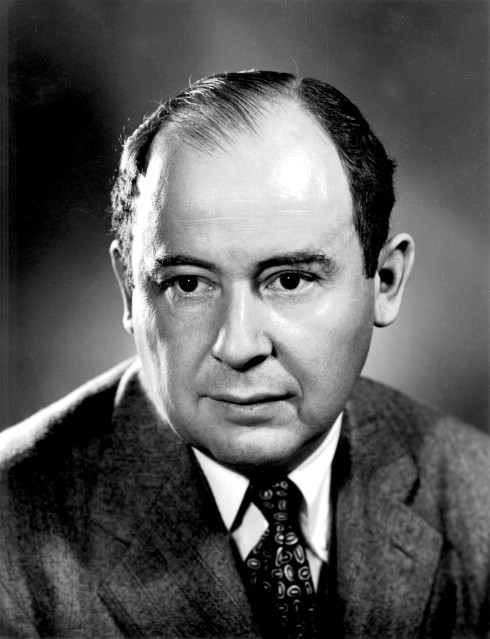
\includegraphics[width=4cm]{von-neuman.jpg}
			John Von Neuman\\
			{\centering\small 1903 - 1957}
		\end{textblock*}
	}

	\begin{frame}{Fenômenos Quânticos}
		\begin{textblock*}{4cm}(2cm, 2cm) % {block width} (coords)
			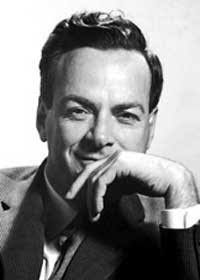
\includegraphics[width=4cm]{feynman.jpg}
			Richard Feynman\\
			{\centering\small 1918 - 1988}
		\end{textblock*}		
	\end{frame}

	\section{Exprimentos}
	\frame{Experimentos}

	\subsection{Algoritmos Quânticos}
	
	\frame%
	{
		\frametitle{Algoritmo de Grover}
		
		\begin{textblock*}{4cm}(2cm, 2.5cm) % {block width} (coords)
			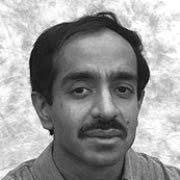
\includegraphics[width=4cm]{grover.jpg}
			Lov Grover\\
			{\centering\small Ex-Bell Labs}
		\end{textblock*}		
	}

	\frame%
	{
		\frametitle{Algoritmo de Shor}
		
		\begin{textblock*}{4cm}(2cm, 2.5cm) % {block width} (coords)
			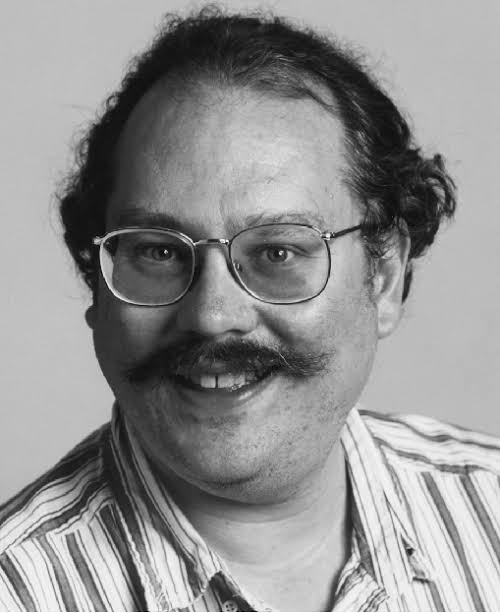
\includegraphics[width=4cm]{shor.jpg}
			Peter Shor\\
			{\centering\small MIT}
		\end{textblock*}		
	}
	
	
	\comicw{quantum-teleportation.pdf}
	
	
	\begin{frame}
		\thebibliography{99}
		\bibitem{shor:94} Shor's Algorithm
	\end{frame}
\end{document}